\chapter{Baseline Forensic Audit and Stage~0 Viterbi Reconstruction}
\label{ch:forensics_viterbi}

This chapter establishes what the local radar benchmark can support before the thesis changes
its signal representation or introduces learned temporal models. It has two linked parts. The first
audits synchronization, reference construction, and session-level error patterns in the frozen
baseline. The second reconstructs a staged set of respiratory-rate trackers, culminating in an
offline Viterbi analysis. Together, these analyses show why a reported rate error is jointly
shaped by the signal, the reference, synchronization, and aggregation rule, and why temporal
continuity alone is not enough to make a tracker trustworthy.

The evidence is intentionally bounded. The frozen baseline can be checked against its own cached
outputs, and the reconstructed methods can be compared on the local cohort variants. The supplied
materials do not identify the original 18 measurement IDs, fully specify the published valid-window
denominator, settle all reference and synchronization details, or specify a complete NMF solver
configuration. Exact reproduction of Beltrão et al. is therefore blocked. The Viterbi results in
this chapter are an internal reconstruction and ablation of the thesis's earlier proposed method;
they are neither a reproduction of an externally published Viterbi system nor a clinical
validation \citep{beltrao2022contactless}.

\section{Provenance, estimands, and the reproduction boundary}
\label{sec:ch3_provenance}

The baseline audit begins with provenance rather than performance. The locked v1 pipeline contains
33 session caches. The independent audit records all 33 as verified against their frozen
checksums. A separate cross-environment parity check reports zero maximum absolute difference in
the DFT, raw-NLS, NMF-NLS, and HPSS-NLS window estimates when the frozen Python 3.9 baseline is
recomputed with the thesis analysis environment. This establishes local computational parity for
the checked artifacts; it does not establish that the local inputs or analysis choices match the
original paper exactly.

That distinction matters because the original study reports 18 retained measurements and
approximately 4,964 valid estimates, whereas the active local \texttt{PAPER\_18} variant contains 5,466
valid two-second windows. Several items needed to reconstruct the original analysis are unresolved:
the original measurement identifiers are not supplied; the reference-target construction and
complete synchronization rule are not uniquely determined; the precise validity gate behind the
published denominator is not recoverable; and the paper does not give a complete
scikit-learn-compatible NMF solver configuration. The present \texttt{PAPER\_18} set is selected using
local reference-validity information, not a verified mapping to the original 18 records. It is
therefore reported as a historical sensitivity analysis, not as the original cohort. The local
NMF comparison also records convergence because a substantial fraction of windows can reach the
iteration cap; the available information does not justify calling that solver identical to the
published solver.

The analysis consequently uses a cohort multiverse rather than treating one locally assembled
subset as definitive. The branch-neutral regime is the primary internal comparison. The other
cohorts expose sensitivity to inclusion rules and the use of the historical 18-measurement subset.

\begin{table}[htbp]
  \centering
  \small
  \caption{Local cohort variants used in the baseline and Stage~0 analyses. Window counts refer
  to valid two-second windows under the branch-neutral synchronization regime.}
  \label{tab:ch3_cohorts}
  \begin{tabular}{@{}lrrl@{}}
    \toprule
    Cohort & Sessions & Valid windows & Role \\
    \midrule
\texttt{all\_paired} & 31 & 7,103 & Broad local sensitivity set \\
\texttt{pool30\_sync} & 28 & 6,640 & Primary internal comparison \\
\texttt{retained23} & 23 & 6,447 & Named-exclusion sensitivity set \\
\texttt{PAPER\_18} & 18 & 5,466 & Historical, locally ranked subset \\
    \bottomrule
  \end{tabular}
\end{table}

The primary error estimand is the equal-session macro-average of session RMSEs,
$\rmseSess= S^{-1}\sum_s \rmseSession{s}$. Each session therefore contributes equally,
regardless of how many valid windows it contains. The window-pooled statistic $\rmsePool$ weights
windows equally and can differ materially. Accuracy is the percentage of valid windows for which
$|e_{s,w}|<\delta$, reported as $\accTau{\delta}$; the threshold is a strict inequality.
Within-session association, $\rWithin$, is the repeated-measures ANCOVA correlation, while
$\rWithinSessMean$ is the unweighted mean of per-session Pearson correlations. These summaries
answer different questions and are not interchangeable. For example, under the cached v1 lag on
\texttt{PAPER\_18}, HPSS has $\rmseSess=6.798$ bpm and $\rmsePool=7.217$ bpm; the mean of per-session
correlations is 0.465, whereas $\rWithin=0.445$.

The cohort-specific LOSO constant predictor is a useful reference for whether a method improves
on predicting a training-derived cohort rate without using the current session's labels. It is
not a sensor and does not define a clinically acceptable error. The session-mean reference SD
oracle is also descriptive: it reports the mean within-session variation of the reference around
each session's mean. Subtracting it from a tracker RMSE gives an oracle-gap diagnostic, not a
universal lower bound on every possible dynamic estimator.

\section{Synchronization audit and the cohort multiverse}
\label{sec:ch3_synchronization}

EXP-0 compares three alignment regimes on the same underlying recordings. In the cached-NMF regime,
the v1 synchronization lag associated with the NMF branch is retained. In the branch-neutral
regime, one shared raw-NLS-derived lag is used for the competing raw, NMF, and HPSS branches. This
prevents a different candidate branch from receiving its own selected lag in the head-to-head
comparison. The lag is still reference-assisted: it comes from the local synchronization workflow
that aligns radar estimates to the one-hertz reference. “Branch-neutral” therefore means shared
across the candidate processing branches, not independent of the reference or outcome. The
pure-metadata regime instead applies the header-clock offset without a correlation search; it is a
clock-only sensitivity analysis, not the primary alignment.

On \texttt{pool30\_sync}, the cached-NMF regime gives HPSS $\rmseSess=8.085$ bpm on 6,642 windows. With
the shared raw-NLS lag, the estimate is 7.817 bpm on 6,640 windows. The LOSO constant baseline is
8.124 bpm and 8.096 bpm in these respective regimes. The corresponding branch-neutral result is
also reproduced in the Stage~0 cache. Across \texttt{all\_paired}, HPSS changes from 8.361 to 8.119 bpm;
on the branch-neutral cohort variants it is 7.973 bpm for \texttt{retained23} and 7.135 bpm for
\texttt{PAPER\_18}. These cohort values are not a ranking of populations: membership, valid-window count,
and—in the historical subset—selection procedure differ.

The small change in valid-window count is material. The cached and branch-neutral \texttt{pool30\_\allowbreak sync}
metrics are not a strict same-windows counterfactual, because changing lag also changes which
windows pass the reference validity and saturation gates. The observed shift is consistent with
branch-specific lag selection affecting the comparison, but the entire difference cannot be
attributed to lag alone. This limitation is particularly clear in Session~12.1: the cached lag is
$-116$ s with 10 valid windows, compared with $-21$ s and 9 valid windows under the shared
raw-NLS lag. HPSS error changes from 18.63 to 3.47 bpm. The local forensic label identifies this
as a lag-pull pattern, but the session also has a large I/Q spread ratio (5.96), I/Q correlation
0.813, and 2.95\% clipped samples. The result shows strong synchronization and gating sensitivity;
it does not show that the physical signal is otherwise clean or isolate lag as the sole cause.

The clock-only regime is substantially worse. On 27 sessions and 6,426 valid windows in
\texttt{pool30\_sync}, HPSS reaches $\rmseSess=10.428$ bpm, compared with a LOSO constant baseline of
8.792 bpm. This indicates that the available header timing alone is not sufficient for this local
comparison. It does not establish that a particular reference-assisted alignment is unbiased;
all such alignment choices should be described as part of the measurement protocol.

\begin{table}[htbp]
  \centering
  \small
  \caption{HPSS baseline under the three synchronization regimes on \texttt{pool30\_sync}. The valid
  window denominator changes with lag and gating; the values are not a same-window lag-only
  contrast.}
  \label{tab:ch3_lag_regimes}
  \begin{tabular}{@{}lrrrr@{}}
    \toprule
    Alignment regime & Sessions & Windows & $\rmseSess$ (bpm) & LOSO constant (bpm) \\
    \midrule
    Cached v1 NMF lag & 28 & 6,642 & 8.085 & 8.124 \\
    Shared raw-NLS lag & 28 & 6,640 & 7.817 & 8.096 \\
    Metadata clock only & 27 & 6,426 & 10.428 & 8.792 \\
    \bottomrule
  \end{tabular}
\end{table}

The broader multiverse gives the same warning against a single headline number. Under the shared
lag, \texttt{all\_paired} yields 8.119 bpm, \texttt{pool30\_sync} 7.817 bpm, \texttt{retained23} 7.973 bpm, and
\texttt{PAPER\_18} 7.135 bpm. The original paper's approximately 4,964 valid estimates are not reproduced
by any of these counts. Cohort and denominator uncertainty remain part of the result rather than
bookkeeping details.

\begin{figure}[htbp]
  \centering
  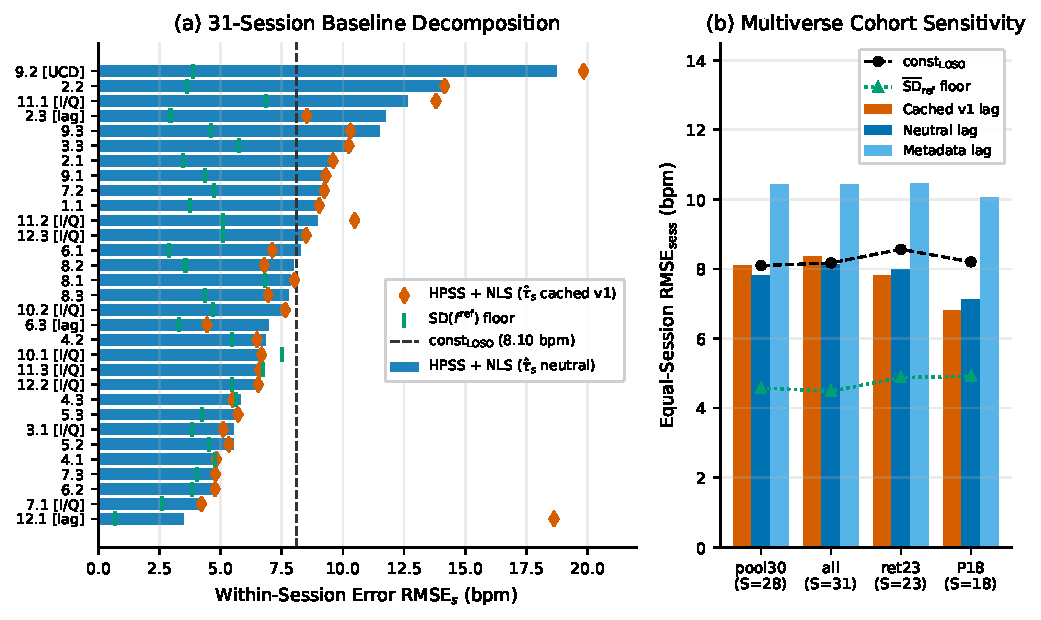
\includegraphics[width=0.92\textwidth]{exp0_session_error_decomposition}
  \caption{Session-wise error under alternative synchronization regimes and local cohort
  definitions. Variation across the panels combines cohort membership, lag, and window validity;
  it should not be read as an isolated causal effect of synchronization.}
  \label{fig:ch3_session_error}
\end{figure}

\section{Reference-channel audit and observed error patterns}
\label{sec:ch3_reference_forensics}

The local EDF contains both a one-hertz \texttt{RespRate} channel and high-rate respiratory trigger
events. These channels represent different constructions of the reference: one is a monitor rate
stream, while the other supports an event-interval estimate. Across 7,101 valid windows, the
1,024-Hz respiratory-trigger rate has a mean signed difference of +2.214 bpm and a mean absolute
difference of 5.175 bpm relative to the one-hertz \texttt{RespRate} channel. The disagreement is not
evidence that either channel is universally correct. A trigger-derived inter-breath rate and a
monitor's smoothed rate can respond differently to pauses, timing, and averaging. It does show
that agreement with the one-hertz channel alone does not fully describe respiratory-event tracking.

The same audit provides a useful channel check: for windows with \texttt{SignalIQ >= 50}, the 1,024-Hz
cardiac R-trigger rate has a 0.935-bpm mean absolute difference from the one-hertz heart-rate
channel across 7,081 windows. This supports the internal consistency of that cardiac trigger
comparison under the stated filter. It does not validate the respiratory trigger as a clinical
ground truth or transfer that validation to the radar estimate.

An inter-trigger gap greater than five seconds flags 1,584 of 7,103 valid windows in the 31-session
neutral-alignment set (22.3\%) and 1,581 of 6,640 windows in \texttt{pool30\_sync} (23.8\%). These are
pause-like intervals defined by the trigger stream. They are not diagnoses of apnea: there is no
clinical adjudication here, and the gating and reference construction affect which intervals are
counted. The distinction matters because an estimator can obtain a lower aggregate error by
rejecting or smoothing windows that contain pauses, even when those intervals may be important to
monitoring.

\begin{figure}[htbp]
  \centering
  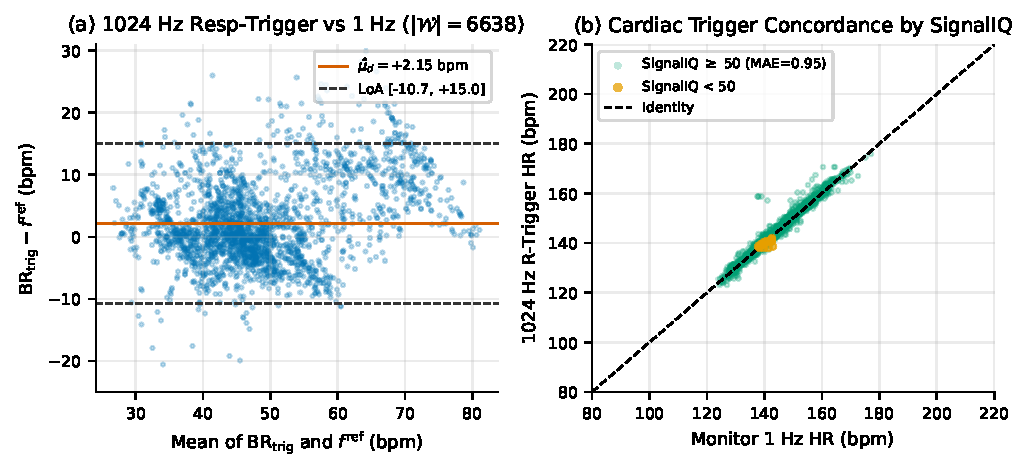
\includegraphics[width=0.92\textwidth]{exp0_edf256_reference_agreement}
  \caption{Agreement between high-rate EDF trigger-derived rates and one-hertz monitor channels.
  The trigger and monitor channels are related references, not interchangeable measurements.}
  \label{fig:ch3_reference_agreement}
\end{figure}

To characterize session error, EXP-0 relates eight telemetry and rate-collision covariates to
excess HPSS error under the shared-lag regime. Here, excess is defined as the session's HPSS RMSE
minus the within-session reference-SD oracle described above. The associations use 28 sessions
from 11 infants and are exploratory Spearman correlations; the listed p-values are nominal and
not adjusted for testing multiple covariates. They identify patterns for follow-up, not causal
effects.

\begin{table}[htbp]
  \centering
  \small
  \caption{Selected exploratory associations with excess session error on \texttt{pool30\_sync}.
  Correlations are across 28 sessions; p-values are nominal and unadjusted.}
  \label{tab:ch3_error_drivers}
  \begin{tabularx}{\textwidth}{@{}Xrrr@{}}
    \toprule
    Session covariate & Spearman $\rho$ with excess error & $p$ & $\rho$ with $\rWithin$ \\
    \midrule
    HR-collision-band window fraction & +0.696 & $<10^{-4}$ & -0.073 \\
    Minimal-movement window fraction & -0.563 & 0.0018 & +0.512 \\
    Windows within 10 bpm of HR/2 & +0.541 & 0.0030 & +0.082 \\
    Respiratory double-octave error fraction & +0.431 & 0.0220 & -0.132 \\
    UCD non-\texttt{ChildPresent} fraction & +0.335 & 0.0810 & -0.112 \\
    \bottomrule
  \end{tabularx}
\end{table}

The strongest positive association is between HR-collision-band windows and excess error. The
negative association with the minimal-movement fraction is consistent with more stable radar
windows being easier to track, but both variables are measured at the session level and can share
other causes. The HR/2 and double-octave patterns are consistent with harmonic ambiguity described
in Chapter~2. The UCD non-child fraction is weaker in this sample and its nominal p-value exceeds
0.05. None of these findings alone shows that cardiac interference, movement, or a device state
caused a specific error. The physics-error and session-decomposition figures are diagnostic
summaries, not interventions.

\begin{figure}[htbp]
  \centering
  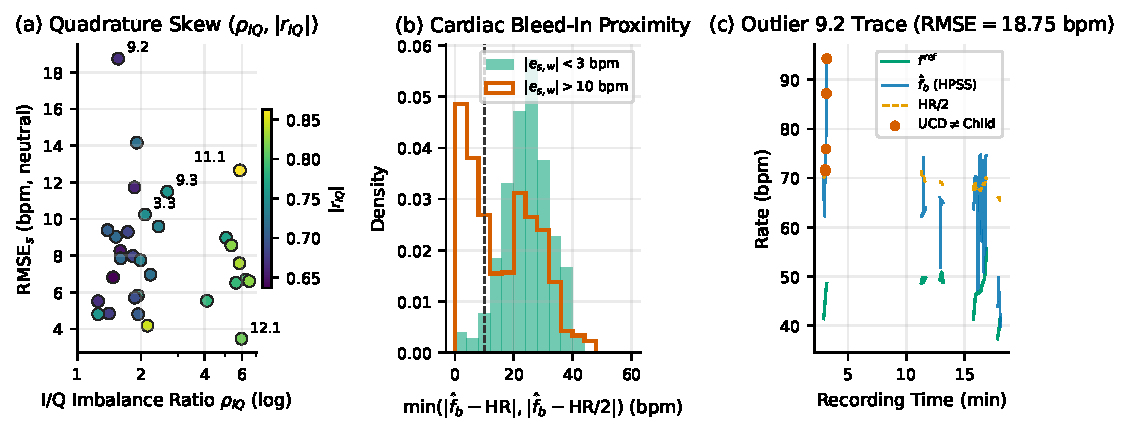
\includegraphics[width=0.92\textwidth]{exp0_physics_error_drivers}
  \caption{Exploratory session-level associations between measured telemetry or rate-collision
  covariates and error. These observational relationships do not identify causal mechanisms.}
  \label{fig:ch3_physics_error}
\end{figure}

Two individual sessions illustrate distinct failure modes that remain after synchronization is
standardized. Session~11.1 has an I/Q standard-deviation ratio of 5.86, absolute I/Q correlation
of 0.863, and clipping in 5.06\% of samples. Its HPSS $\rmseSess$ is 12.65 bpm with the shared
lag, 13.81 bpm under the cached lag, and 16.22 bpm under metadata-only timing. A large spread
imbalance, collinearity, and clipping can make a quadrature trajectory poorly conditioned, but
these measurements do not identify which receiver or motion mechanism dominates the error.

Session~9.2 has an observed mid-session UCD status dropout from \texttt{ChildPresent}. Under the shared
lag its HPSS error is 18.75 bpm; metadata-only timing gives 11.68 bpm. This contrast cautions
against treating the status flag as a sufficient quality score or assuming one lag regime corrects
every session. Telemetry and status fields are contextual indicators, not ground-truth labels for
the failure mechanism.

\section{Stage~0: reconstruction of score-based Viterbi tracking}
\label{sec:ch3_viterbi_methods}

Stage~0 asks whether sequence decoding improves the locked HPSS-NLS baseline and which ingredients
are needed for any improvement. The comparison is performed on \texttt{pool30\_sync}, using the shared
raw-NLS-derived lag and the one-hertz respiratory-rate reference. It contains 28 sessions from 11
infants and 6,640 valid windows. \texttt{A4\_HPSS\_NLS} is the frozen signal-processing anchor. DFT, raw
NLS, and NMF-NLS baselines separate the contributions of a spectral peak, harmonic scoring, and
NMF preprocessing. The B-series explores alternative spectral evidence; the C-series adds
one-dimensional or joint breathing--heart-rate states, harmonic-aware penalties, and
leave-one-patient-out (LOPO) transition selection.

For each window, the tracker receives a score over a discrete breathing-rate grid. The basic
one-dimensional model uses candidate rates from 18 to 90 bpm at 2-bpm spacing. A transition term
penalizes large adjacent rate changes with a Gaussian-shaped log score. The Viterbi recursion
maximizes the summed emission and transition scores over the complete sequence. The two-dimensional
variant adds a heart-rate state on a 90--210 bpm grid and a harmonic-quality term that penalizes
breathing candidates that collide with plausible cardiac harmonics. It is a joint latent-state
decoder; it should not be interpreted as a validated heart-rate output.

The ablations distinguish two design choices that can otherwise be confounded. Unanchored spectral
emissions use broad Welch or harmonic-NLS evidence directly. Anchored emissions use a coarse
autocorrelation estimate to weight harmonic evidence near a local candidate. The latter retains
the temporal optimizer but gives it a physiologically informed local reference. LOPO variants
select transition and emission settings on training patients while holding out the test patient.
The selected parameters are therefore not fitted to that patient's evaluation labels, although
the decoded path itself still uses the full held-out session and is offline.

The anchored harmonic-NLS peak baseline (\texttt{B5a}) reaches 7.701 bpm equal-session RMSE,
compared with 7.817 bpm for \texttt{A4\_HPSS\_NLS}. This modest difference shows that local
anchoring changes the candidate evidence even before sequence decoding. The Viterbi ablations
then test whether temporal structure improves that anchored representation.

\begin{table}[htbp]
  \centering
  \small
  \caption{Representative Stage~0 methods on \texttt{pool30\_sync} with the shared lag. $\Delta$ is
  the change in equal-session RMSE relative to \texttt{A4\_HPSS\_NLS}; negative values favor the method.}
  \label{tab:ch3_viterbi_ladder}
  \begin{tabular}{@{}lrrrrr@{}}
    \toprule
    Method & $\rmseSess$ & $\rmsePool$ & $\accTau{10}$ & $\rWithin$ & $\Delta$ \\
    & bpm & bpm & \% & & bpm \\
    \midrule
    A1 DFT & 11.878 & 11.459 & 65.1 & 0.353 & +4.061 \\
    A2 raw NLS & 8.172 & 8.021 & 77.1 & 0.466 & +0.355 \\
    A3 NMF-NLS & 8.074 & 8.146 & 79.1 & 0.377 & +0.256 \\
    A4 HPSS-NLS & 7.817 & 7.970 & 79.4 & 0.423 & 0.000 \\
    B5a anchored harmonic-NLS peak & 7.701 & 7.887 & 79.3 & 0.431 & -0.116 \\
    C1b 1D Welch Viterbi & 10.109 & 10.219 & 70.7 & 0.361 & +2.292 \\
    C2b 1D HQI Viterbi & 10.077 & 10.160 & 70.4 & 0.369 & +2.259 \\
    C3b joint BR/HR Viterbi & 9.648 & 9.923 & 72.3 & 0.359 & +1.831 \\
    C4b unanchored harmonic-NLS Viterbi & 13.030 & 14.344 & 55.9 & 0.159 & +5.213 \\
    C4c anchored 1D Viterbi & 7.182 & 7.513 & 81.6 & 0.452 & -0.636 \\
    C4d anchored joint Viterbi & 7.036 & 7.306 & 82.0 & 0.471 & -0.782 \\
    C6d LOPO wide anchored Viterbi & 6.877 & 7.205 & 83.7 & 0.456 & -0.941 \\
    \bottomrule
  \end{tabular}
\end{table}

The unanchored sequence models do not improve the baseline. The 1D Welch Viterbi has an equal-
session RMSE of 10.109 bpm, and the joint BR/HR model has 9.648 bpm, both worse than the
7.817-bpm \texttt{A4\_HPSS\_NLS} anchor. Adding unanchored harmonic-NLS evidence alone is not sufficient:
\texttt{C4b} reaches 13.030 bpm. These results oppose the simple hypothesis that a temporal prior or a
larger joint state space automatically resolves harmonic confusion. When the emission surface
places strong mass on a half-rate, double-rate, or cardiac-related candidate, sequence continuity
can preserve the wrong path over time.

Anchoring the harmonic evidence changes the result. Beyond the \texttt{B5a} anchored peak baseline,
\texttt{C4c} reduces $\rmseSess$ to 7.182 bpm, and the joint anchored \texttt{C4d} reaches 7.036
bpm. The \texttt{C6d} LOPO-wide transition variant reaches 6.877
bpm, with a paired mean difference from \texttt{A4} of $-0.941$ bpm. It wins on all 11 patient-level
aggregates; the patient-level Wilcoxon comparison remains significant after the reported Holm
correction ($p_{\mathrm{pat,Holm}}=0.0205$). This is internal evidence for the tested
branch-neutral cohort and reference, not evidence of generalization to an unseen site or bedside
benefit. \texttt{C6e}, the corresponding NMF variant, has a slightly lower point RMSE of 6.826 bpm, but
its result also depends on the incompletely specified local NMF solver and is not the primary
HPSS reconstruction.

The LOPO analysis has a further selection boundary. The wide search evaluates a finite grid of
one- and two-dimensional settings, and \texttt{C6d} selects a boundary-valued configuration in all 11
folds (none is upper-pinned; all are flagged as a boundary selection). This does not invalidate the
held-patient comparison, but it means the grid did not locate an interior optimum. The result is
best read as performance among the prespecified candidates, with transition settings that merit
further search or regularization.

\begin{figure}[htbp]
  \centering
  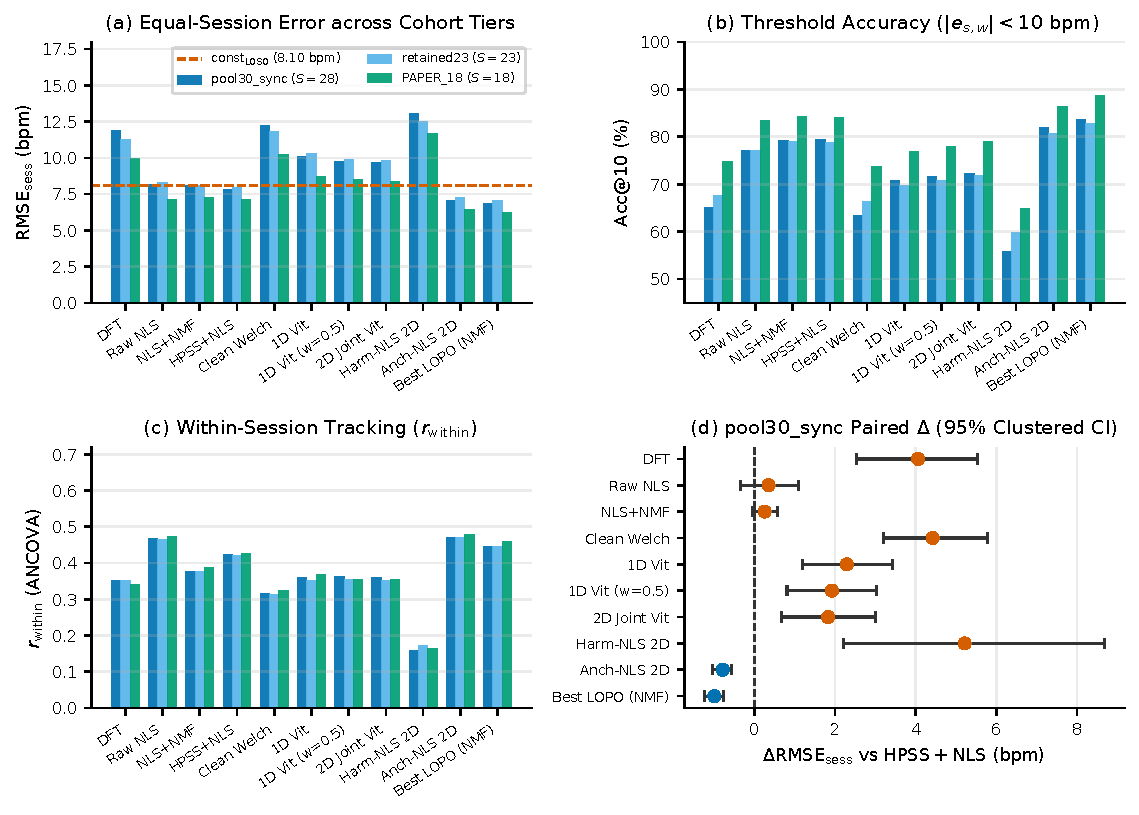
\includegraphics[width=0.92\textwidth]{viterbi_repro_ablation_ladder}
  \caption{Stage~0 ablation ladder. Unanchored sequence decoding degrades the baseline, whereas
  anchored harmonic evidence recovers lower error on the tested local cohort.}
  \label{fig:ch3_ablation_ladder}
\end{figure}

\begin{figure}[htbp]
  \centering
  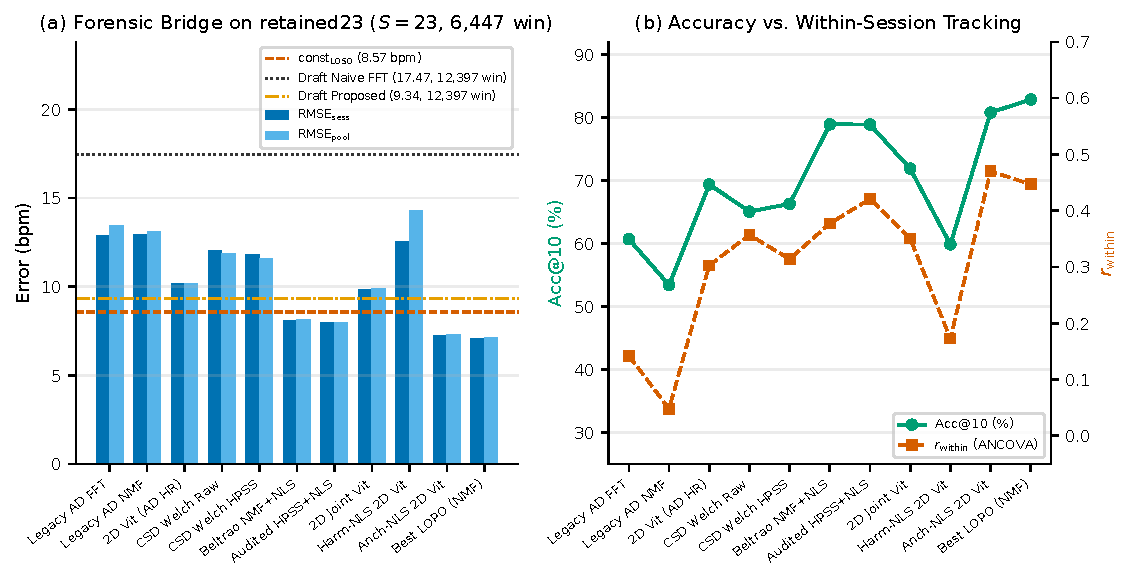
\includegraphics[width=0.92\textwidth]{viterbi_repro_forensic_bridge}
  \caption{Forensic bridge from the signal-processing baseline to Viterbi variants, including
  the role of candidate evidence and temporal structure.}
  \label{fig:ch3_forensic_bridge}
\end{figure}

\section{Agreement, negative controls, and the offline limit}
\label{sec:ch3_viterbi_controls}

RMSE is not a sufficient description of a tracker. A path can reduce average error while losing
dynamic association with the reference, and pooled-window metrics can conceal session-level
disagreement. The reconstructed analysis therefore reports equal-session and pooled RMSE,
within-session correlation, strict-threshold accuracy, and Bland--Altman summaries separately.
On \texttt{PAPER\_18}, the difference between $\rmseSess$ and $\rmsePool$ is about 0.42 bpm for the
cached HPSS baseline, illustrating why the aggregation rule must accompany a result.

The surrogate controls test whether a favorable metric can persist when the temporal or radar
structure is disrupted. In 20 time-shuffled-reference runs, within-session correlations for the
baseline and representative Viterbi methods are approximately zero. In five full-session
phase-scrambled-radar runs, the anchored joint Viterbi likewise has near-zero mean within-session
correlation (approximately $-0.001$), despite a finite aggregate RMSE. Phase scrambling preserves
the session Fourier magnitudes while randomizing phase; it is a stress test of the signal's
temporal structure, not a model of a particular clinical artifact. The near-zero association
shows why a plausible-looking rate range or aggregate error alone cannot establish that a method
is following respiratory information.

A stiff-transition control makes the same point from another direction. With the breathing-rate
transition scale forced to 0.25 bpm, an anchored 2D tracker reports $\rmseSess=6.188$ bpm, lower
than \texttt{C6d}, but its $\rWithin$ is only 0.266. A very strong temporal prior can compress changes
and improve average error on a restricted sample while tracking less of the within-session
variation. This control argues against selecting a tracker from RMSE alone.

Synthetic checks support implementation behavior under constructed conditions, with limits. The
anchored 2D tracker returns the exact 45-bpm state in the stationary 45-bpm/150-bpm-heart-rate
example. In the constructed 35-to-65-bpm chirp with movement and a 150-bpm cardiac component, its
RMSE is approximately 0.326 bpm. These results show that the tested code can resolve those
specified synthetic mixtures; they do not establish that real neonatal signals follow the same
model or that the method handles unmodeled movement and reference error.

The HR component of the joint state was also evaluated against the high-rate R-trigger reference
as a separate output. None of nine cardiac extractors passes the predefined 50\% within-10-bpm
criterion; the best session-averaged result is 39.8\%. Thus, the HR state in the joint decoder is
used as auxiliary evidence for harmonic ambiguity. The present analysis does not validate it as a
clinical heart-rate measurement.

Finally, Stage~0 Viterbi decoding is noncausal. The optimal path is recovered by backtracking from
the final frame, so each estimate can depend on future observations from the full processed
session. The LOPO split protects patient-level parameter selection, but it does not turn this
offline path into a zero-lookahead estimate. The improvements therefore motivate the constrained
causal filters in Chapter~4; they do not demonstrate real-time tracking, alarm latency, or bedside
apnea detection.

\begin{figure}[htbp]
  \centering
  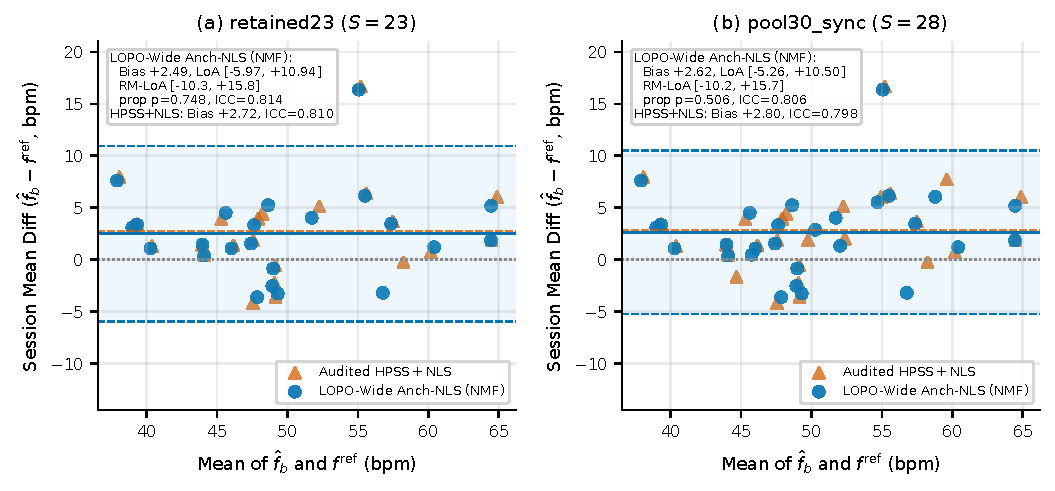
\includegraphics[width=0.92\textwidth]{viterbi_repro_bland_altman}
  \caption{Agreement summaries for representative Stage~0 methods. Limits and bias are shown
  with session structure retained; correlation alone would not characterize this agreement.}
  \label{fig:ch3_bland_altman}
\end{figure}

\begin{figure}[htbp]
  \centering
  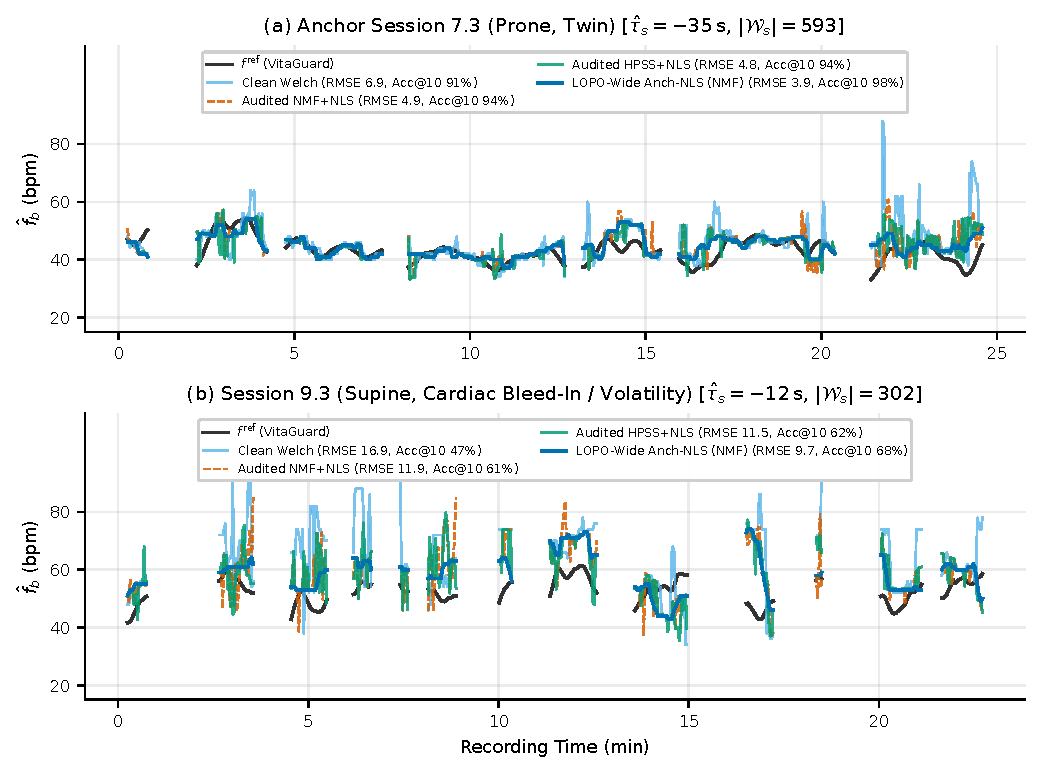
\includegraphics[width=0.92\textwidth]{viterbi_repro_tracking_examples}
  \caption{Example tracking trajectories illustrating candidate selection and temporal
  continuity. These selected sessions illustrate mechanisms and are not a substitute for the
  cohort-level summaries.}
  \label{fig:ch3_tracking_examples}
\end{figure}

\section{Chapter summary}
\label{sec:ch3_summary}

This chapter verified the local baseline caches and reconstructed the main Stage~0 comparisons,
while maintaining the distinction between internal parity and exact paper reproduction. The
reference-assisted shared lag reduces branch-specific alignment differences but does not remove
reference dependence, and lag changes also alter the valid-window denominator. Across the local
cohort variants, session-level error varies with inclusion and synchronization. Exploratory
session correlations point to cardiac-rate collisions and movement-related measures as useful
diagnostic leads, but they do not identify causes. Trigger-versus-monitor disagreement further
shows that the reference itself has a measurement definition and time scale.

The Viterbi ablation gives a more specific methodological result. Unanchored Viterbi and joint
BR/HR decoding worsen the baseline; anchored harmonic emissions recover better internal error,
with the best reported LOPO-wide HPSS model at 6.877 bpm. That result is bounded by 11 infants,
reference-assisted synchronization, boundary selections in every LOPO fold, and offline
infinite-lookahead decoding. The surrogate controls also show that low aggregate error can coexist
with almost no within-session association after signal structure is disrupted. Chapter~4 therefore
tests causal, constrained alternatives and their front-end assumptions, rather than treating the
offline Stage~0 optimum as a deployable monitor.
